% Options for packages loaded elsewhere
\PassOptionsToPackage{unicode}{hyperref}
\PassOptionsToPackage{hyphens}{url}
\PassOptionsToPackage{dvipsnames,svgnames,x11names}{xcolor}
%
\documentclass[
  letterpaper,
  DIV=11]{scrartcl}

\usepackage{amsmath,amssymb}
\usepackage{iftex}
\ifPDFTeX
  \usepackage[T1]{fontenc}
  \usepackage[utf8]{inputenc}
  \usepackage{textcomp} % provide euro and other symbols
\else % if luatex or xetex
  \usepackage{unicode-math}
  \defaultfontfeatures{Scale=MatchLowercase}
  \defaultfontfeatures[\rmfamily]{Ligatures=TeX,Scale=1}
\fi
\usepackage{lmodern}
\ifPDFTeX\else  
    % xetex/luatex font selection
\fi
% Use upquote if available, for straight quotes in verbatim environments
\IfFileExists{upquote.sty}{\usepackage{upquote}}{}
\IfFileExists{microtype.sty}{% use microtype if available
  \usepackage[]{microtype}
  \UseMicrotypeSet[protrusion]{basicmath} % disable protrusion for tt fonts
}{}
\makeatletter
\@ifundefined{KOMAClassName}{% if non-KOMA class
  \IfFileExists{parskip.sty}{%
    \usepackage{parskip}
  }{% else
    \setlength{\parindent}{0pt}
    \setlength{\parskip}{6pt plus 2pt minus 1pt}}
}{% if KOMA class
  \KOMAoptions{parskip=half}}
\makeatother
\usepackage{xcolor}
\setlength{\emergencystretch}{3em} % prevent overfull lines
\setcounter{secnumdepth}{5}
% Make \paragraph and \subparagraph free-standing
\ifx\paragraph\undefined\else
  \let\oldparagraph\paragraph
  \renewcommand{\paragraph}[1]{\oldparagraph{#1}\mbox{}}
\fi
\ifx\subparagraph\undefined\else
  \let\oldsubparagraph\subparagraph
  \renewcommand{\subparagraph}[1]{\oldsubparagraph{#1}\mbox{}}
\fi

\usepackage{color}
\usepackage{fancyvrb}
\newcommand{\VerbBar}{|}
\newcommand{\VERB}{\Verb[commandchars=\\\{\}]}
\DefineVerbatimEnvironment{Highlighting}{Verbatim}{commandchars=\\\{\}}
% Add ',fontsize=\small' for more characters per line
\usepackage{framed}
\definecolor{shadecolor}{RGB}{241,243,245}
\newenvironment{Shaded}{\begin{snugshade}}{\end{snugshade}}
\newcommand{\AlertTok}[1]{\textcolor[rgb]{0.68,0.00,0.00}{#1}}
\newcommand{\AnnotationTok}[1]{\textcolor[rgb]{0.37,0.37,0.37}{#1}}
\newcommand{\AttributeTok}[1]{\textcolor[rgb]{0.40,0.45,0.13}{#1}}
\newcommand{\BaseNTok}[1]{\textcolor[rgb]{0.68,0.00,0.00}{#1}}
\newcommand{\BuiltInTok}[1]{\textcolor[rgb]{0.00,0.23,0.31}{#1}}
\newcommand{\CharTok}[1]{\textcolor[rgb]{0.13,0.47,0.30}{#1}}
\newcommand{\CommentTok}[1]{\textcolor[rgb]{0.37,0.37,0.37}{#1}}
\newcommand{\CommentVarTok}[1]{\textcolor[rgb]{0.37,0.37,0.37}{\textit{#1}}}
\newcommand{\ConstantTok}[1]{\textcolor[rgb]{0.56,0.35,0.01}{#1}}
\newcommand{\ControlFlowTok}[1]{\textcolor[rgb]{0.00,0.23,0.31}{#1}}
\newcommand{\DataTypeTok}[1]{\textcolor[rgb]{0.68,0.00,0.00}{#1}}
\newcommand{\DecValTok}[1]{\textcolor[rgb]{0.68,0.00,0.00}{#1}}
\newcommand{\DocumentationTok}[1]{\textcolor[rgb]{0.37,0.37,0.37}{\textit{#1}}}
\newcommand{\ErrorTok}[1]{\textcolor[rgb]{0.68,0.00,0.00}{#1}}
\newcommand{\ExtensionTok}[1]{\textcolor[rgb]{0.00,0.23,0.31}{#1}}
\newcommand{\FloatTok}[1]{\textcolor[rgb]{0.68,0.00,0.00}{#1}}
\newcommand{\FunctionTok}[1]{\textcolor[rgb]{0.28,0.35,0.67}{#1}}
\newcommand{\ImportTok}[1]{\textcolor[rgb]{0.00,0.46,0.62}{#1}}
\newcommand{\InformationTok}[1]{\textcolor[rgb]{0.37,0.37,0.37}{#1}}
\newcommand{\KeywordTok}[1]{\textcolor[rgb]{0.00,0.23,0.31}{#1}}
\newcommand{\NormalTok}[1]{\textcolor[rgb]{0.00,0.23,0.31}{#1}}
\newcommand{\OperatorTok}[1]{\textcolor[rgb]{0.37,0.37,0.37}{#1}}
\newcommand{\OtherTok}[1]{\textcolor[rgb]{0.00,0.23,0.31}{#1}}
\newcommand{\PreprocessorTok}[1]{\textcolor[rgb]{0.68,0.00,0.00}{#1}}
\newcommand{\RegionMarkerTok}[1]{\textcolor[rgb]{0.00,0.23,0.31}{#1}}
\newcommand{\SpecialCharTok}[1]{\textcolor[rgb]{0.37,0.37,0.37}{#1}}
\newcommand{\SpecialStringTok}[1]{\textcolor[rgb]{0.13,0.47,0.30}{#1}}
\newcommand{\StringTok}[1]{\textcolor[rgb]{0.13,0.47,0.30}{#1}}
\newcommand{\VariableTok}[1]{\textcolor[rgb]{0.07,0.07,0.07}{#1}}
\newcommand{\VerbatimStringTok}[1]{\textcolor[rgb]{0.13,0.47,0.30}{#1}}
\newcommand{\WarningTok}[1]{\textcolor[rgb]{0.37,0.37,0.37}{\textit{#1}}}

\providecommand{\tightlist}{%
  \setlength{\itemsep}{0pt}\setlength{\parskip}{0pt}}\usepackage{longtable,booktabs,array}
\usepackage{calc} % for calculating minipage widths
% Correct order of tables after \paragraph or \subparagraph
\usepackage{etoolbox}
\makeatletter
\patchcmd\longtable{\par}{\if@noskipsec\mbox{}\fi\par}{}{}
\makeatother
% Allow footnotes in longtable head/foot
\IfFileExists{footnotehyper.sty}{\usepackage{footnotehyper}}{\usepackage{footnote}}
\makesavenoteenv{longtable}
\usepackage{graphicx}
\makeatletter
\def\maxwidth{\ifdim\Gin@nat@width>\linewidth\linewidth\else\Gin@nat@width\fi}
\def\maxheight{\ifdim\Gin@nat@height>\textheight\textheight\else\Gin@nat@height\fi}
\makeatother
% Scale images if necessary, so that they will not overflow the page
% margins by default, and it is still possible to overwrite the defaults
% using explicit options in \includegraphics[width, height, ...]{}
\setkeys{Gin}{width=\maxwidth,height=\maxheight,keepaspectratio}
% Set default figure placement to htbp
\makeatletter
\def\fps@figure{htbp}
\makeatother

\KOMAoption{captions}{tableheading}
\makeatletter
\makeatother
\makeatletter
\makeatother
\makeatletter
\@ifpackageloaded{caption}{}{\usepackage{caption}}
\AtBeginDocument{%
\ifdefined\contentsname
  \renewcommand*\contentsname{Inhaltsverzeichnis}
\else
  \newcommand\contentsname{Inhaltsverzeichnis}
\fi
\ifdefined\listfigurename
  \renewcommand*\listfigurename{Abbildungsverzeichnis}
\else
  \newcommand\listfigurename{Abbildungsverzeichnis}
\fi
\ifdefined\listtablename
  \renewcommand*\listtablename{Tabellenverzeichnis}
\else
  \newcommand\listtablename{Tabellenverzeichnis}
\fi
\ifdefined\figurename
  \renewcommand*\figurename{Abbildung}
\else
  \newcommand\figurename{Abbildung}
\fi
\ifdefined\tablename
  \renewcommand*\tablename{Tabelle}
\else
  \newcommand\tablename{Tabelle}
\fi
}
\@ifpackageloaded{float}{}{\usepackage{float}}
\floatstyle{ruled}
\@ifundefined{c@chapter}{\newfloat{codelisting}{h}{lop}}{\newfloat{codelisting}{h}{lop}[chapter]}
\floatname{codelisting}{Listing}
\newcommand*\listoflistings{\listof{codelisting}{Listingverzeichnis}}
\makeatother
\makeatletter
\@ifpackageloaded{caption}{}{\usepackage{caption}}
\@ifpackageloaded{subcaption}{}{\usepackage{subcaption}}
\makeatother
\makeatletter
\@ifpackageloaded{tcolorbox}{}{\usepackage[skins,breakable]{tcolorbox}}
\makeatother
\makeatletter
\@ifundefined{shadecolor}{\definecolor{shadecolor}{rgb}{.97, .97, .97}}
\makeatother
\makeatletter
\makeatother
\makeatletter
\makeatother
\ifLuaTeX
\usepackage[bidi=basic]{babel}
\else
\usepackage[bidi=default]{babel}
\fi
\babelprovide[main,import]{ngerman}
% get rid of language-specific shorthands (see #6817):
\let\LanguageShortHands\languageshorthands
\def\languageshorthands#1{}
\ifLuaTeX
  \usepackage{selnolig}  % disable illegal ligatures
\fi
\IfFileExists{bookmark.sty}{\usepackage{bookmark}}{\usepackage{hyperref}}
\IfFileExists{xurl.sty}{\usepackage{xurl}}{} % add URL line breaks if available
\urlstyle{same} % disable monospaced font for URLs
\hypersetup{
  pdftitle={Einkaufsgewohnheiten in den USA},
  pdfauthor={Ole Kepa,  Fabian Elsner,  Sören Bax},
  pdflang={de},
  colorlinks=true,
  linkcolor={blue},
  filecolor={Maroon},
  citecolor={Blue},
  urlcolor={Blue},
  pdfcreator={LaTeX via pandoc}}

\title{Einkaufsgewohnheiten in den USA}
\author{Ole Kepa, Fabian Elsner, Sören Bax}
\date{}

\begin{document}
\maketitle
\ifdefined\Shaded\renewenvironment{Shaded}{\begin{tcolorbox}[interior hidden, borderline west={3pt}{0pt}{shadecolor}, frame hidden, breakable, enhanced, boxrule=0pt, sharp corners]}{\end{tcolorbox}}\fi

\renewcommand*\contentsname{Inhaltsverzeichnis}
{
\hypersetup{linkcolor=}
\setcounter{tocdepth}{3}
\tableofcontents
}
\hypertarget{gendererkluxe4rung}{%
\section{Gendererklärung}\label{gendererkluxe4rung}}

Aus Lesbarkeitsgründen wird in dieser Studienarbeit auf die verschiedene
Ansprechweisen, sei es divers, männlich oder weiblich verzichtet. Alle
Formulierungen sprechen gleichermaßen alle Geschlechter an.

\hypertarget{aufgabe-und-daten-verstehen}{%
\section{Aufgabe und Daten
verstehen}\label{aufgabe-und-daten-verstehen}}

\hypertarget{beschreibung-der-datenquelle}{%
\section{Beschreibung der
Datenquelle}\label{beschreibung-der-datenquelle}}

Laden wir zuerst die beiden Datensets:

\begin{Shaded}
\begin{Highlighting}[]
\NormalTok{shopping\_trends }\OtherTok{\textless{}{-}} \FunctionTok{read\_csv}\NormalTok{(}\StringTok{\textquotesingle{}./data/shopping\_trends.csv\textquotesingle{}}\NormalTok{)}
\NormalTok{shopping\_behavior }\OtherTok{\textless{}{-}} \FunctionTok{read\_csv}\NormalTok{(}\StringTok{\textquotesingle{}./data/shopping\_behavior\_updated.csv\textquotesingle{}}\NormalTok{)}
\end{Highlighting}
\end{Shaded}

Nun werfen wir einen kurzen Blick auf die Datenstrukturen. Zunächst
einmal die Datenstruktur des Datensets ``Shopping\_trends'':

\begin{Shaded}
\begin{Highlighting}[]
\NormalTok{shopping\_trends}
\end{Highlighting}
\end{Shaded}

\begin{verbatim}
# A tibble: 3,900 x 19
   `Customer ID`   Age Gender `Item Purchased` Category   Purchase Amount (USD~1
           <dbl> <dbl> <chr>  <chr>            <chr>                       <dbl>
 1             1    55 Male   Blouse           Clothing                       53
 2             2    19 Male   Sweater          Clothing                       64
 3             3    50 Male   Jeans            Clothing                       73
 4             4    21 Male   Sandals          Footwear                       90
 5             5    45 Male   Blouse           Clothing                       49
 6             6    46 Male   Sneakers         Footwear                       20
 7             7    63 Male   Shirt            Clothing                       85
 8             8    27 Male   Shorts           Clothing                       34
 9             9    26 Male   Coat             Outerwear                      97
10            10    57 Male   Handbag          Accessori~                     31
# i 3,890 more rows
# i abbreviated name: 1: `Purchase Amount (USD)`
# i 13 more variables: Location <chr>, Size <chr>, Color <chr>, Season <chr>,
#   `Review Rating` <dbl>, `Subscription Status` <chr>, `Payment Method` <chr>,
#   `Shipping Type` <chr>, `Discount Applied` <chr>, `Promo Code Used` <chr>,
#   `Previous Purchases` <dbl>, `Preferred Payment Method` <chr>,
#   `Frequency of Purchases` <chr>
\end{verbatim}

Jede Zeile steht für einen *********

\begin{longtable}[]{@{}
  >{\raggedright\arraybackslash}p{(\columnwidth - 4\tabcolsep) * \real{0.3590}}
  >{\raggedright\arraybackslash}p{(\columnwidth - 4\tabcolsep) * \real{0.0897}}
  >{\raggedright\arraybackslash}p{(\columnwidth - 4\tabcolsep) * \real{0.5513}}@{}}
\toprule\noalign{}
\begin{minipage}[b]{\linewidth}\raggedright
Variable
\end{minipage} & \begin{minipage}[b]{\linewidth}\raggedright
Typ
\end{minipage} & \begin{minipage}[b]{\linewidth}\raggedright
Bedeutung
\end{minipage} \\
\midrule\noalign{}
\endhead
\bottomrule\noalign{}
\endlastfoot
\textbf{Customer ID} & dbl & Eindeutige Kunden Identifikationsnummer \\
\textbf{Age} & dbl & Alter des Kundens \\
\textbf{Gender} & chr & Geschlecht des Kundens \\
\textbf{Item Purchased} & chr & Gekauftes Produkt \\
\textbf{Category} & chr & Kategorie des gekauften Produkts \\
\textbf{Purchase Amount} & dbl & Bezahlter Preis \\
\textbf{Location} & chr & \\
\textbf{Size} & chr & \\
\textbf{Color} & chr & \\
\textbf{Season} & chr & \\
\textbf{Review Rating} & dbl & \\
\textbf{Subscription Status} & chr & \\
\textbf{Payment Method} & chr & \\
\textbf{Shipping Type} & chr & \\
\textbf{Discount Applied} & chr & \\
\textbf{Promo Code Used} & chr & \\
\textbf{Previous Purchases} & dbl & \\
\textbf{Preferred Payment Method} & chr & \\
\textbf{Frequency of Purchases} & chr & \\
\end{longtable}

\begin{Shaded}
\begin{Highlighting}[]
\FunctionTok{describe\_tbl}\NormalTok{(shopping\_trends)}
\end{Highlighting}
\end{Shaded}

\begin{verbatim}
3 900 (3.9k) observations with 19 variables
0 observations containing missings (NA)
0 variables containing missings (NA)
0 variables with no variance
\end{verbatim}

Im Datensatz ``Shopping\_trends'' gibt es 3.900 Instazen
(Beobachtungen). Keine dieser Instanzen enthalten Werte ohne Angabe
(NA), daher müssen wir das Datenset nicht aufgrund fehlender Variablen
aufbereiten. Nun schauen wir auf die Datenstruktur des Datensets
``Shopping\_behavior'':

\begin{Shaded}
\begin{Highlighting}[]
\NormalTok{shopping\_behavior}
\end{Highlighting}
\end{Shaded}

\begin{verbatim}
# A tibble: 3,900 x 18
   `Customer ID`   Age Gender `Item Purchased` Category   Purchase Amount (USD~1
           <dbl> <dbl> <chr>  <chr>            <chr>                       <dbl>
 1             1    55 Male   Blouse           Clothing                       53
 2             2    19 Male   Sweater          Clothing                       64
 3             3    50 Male   Jeans            Clothing                       73
 4             4    21 Male   Sandals          Footwear                       90
 5             5    45 Male   Blouse           Clothing                       49
 6             6    46 Male   Sneakers         Footwear                       20
 7             7    63 Male   Shirt            Clothing                       85
 8             8    27 Male   Shorts           Clothing                       34
 9             9    26 Male   Coat             Outerwear                      97
10            10    57 Male   Handbag          Accessori~                     31
# i 3,890 more rows
# i abbreviated name: 1: `Purchase Amount (USD)`
# i 12 more variables: Location <chr>, Size <chr>, Color <chr>, Season <chr>,
#   `Review Rating` <dbl>, `Subscription Status` <chr>, `Shipping Type` <chr>,
#   `Discount Applied` <chr>, `Promo Code Used` <chr>,
#   `Previous Purchases` <dbl>, `Payment Method` <chr>,
#   `Frequency of Purchases` <chr>
\end{verbatim}

Jede Zeile steht für *******.

\begin{longtable}[]{@{}
  >{\raggedright\arraybackslash}p{(\columnwidth - 4\tabcolsep) * \real{0.3889}}
  >{\raggedright\arraybackslash}p{(\columnwidth - 4\tabcolsep) * \real{0.0972}}
  >{\raggedright\arraybackslash}p{(\columnwidth - 4\tabcolsep) * \real{0.5139}}@{}}
\toprule\noalign{}
\begin{minipage}[b]{\linewidth}\raggedright
Variable
\end{minipage} & \begin{minipage}[b]{\linewidth}\raggedright
Typ
\end{minipage} & \begin{minipage}[b]{\linewidth}\raggedright
Bedeutung
\end{minipage} \\
\midrule\noalign{}
\endhead
\bottomrule\noalign{}
\endlastfoot
\textbf{Customer ID} & dbl & Eindeutige Kunden Identifikationsnummer \\
\textbf{Age} & dbl & Alter des Kundens \\
\textbf{Gender} & chr & Geschlecht des Kundens \\
\textbf{Item Purchased} & chr & Gekauftes Produkt \\
\textbf{Category} & chr & Kategorie des gekauften Produkts \\
\textbf{Purchase Amount} & dbl & Bezahlter Preis \\
\textbf{Location} & chr & \\
\textbf{Size} & chr & \\
\textbf{Color} & chr & \\
\textbf{Season} & chr & \\
\textbf{Review Rating} & dbl & \\
\textbf{Subscription Status} & chr & \\
\textbf{Payment Method} & chr & \\
\textbf{Shipping Type} & chr & \\
\textbf{Discount Applied} & chr & \\
\textbf{Promo Code Used} & chr & \\
\textbf{Previous Purchases} & dbl & \\
\textbf{Payment Method} & chr & \\
\textbf{Frequency of Purchases} & chr & \\
\end{longtable}

\begin{Shaded}
\begin{Highlighting}[]
\FunctionTok{describe\_tbl}\NormalTok{(shopping\_behavior)}
\end{Highlighting}
\end{Shaded}

\begin{verbatim}
3 900 (3.9k) observations with 18 variables
0 observations containing missings (NA)
0 variables containing missings (NA)
0 variables with no variance
\end{verbatim}

Im Datensatz ``Shoping\_behavior'' gibt es ebenfalls 3.900 Instazen
(Beobachtungen). Zudem gibt wa qiwswe bwi jwswe Instanz keine enthalten
Werte ohne Angabe (NA). Daher müssen wir, wie beim vorherigen Datensatz
keine fehlenden Variablen aufbereiten.

\hypertarget{untersuchung-der-daten-auf-ausreiuxdfer}{%
\section{Untersuchung der Daten (Auf
ausreißer)}\label{untersuchung-der-daten-auf-ausreiuxdfer}}

\hypertarget{untersuchung-der-thesen-mit-methoden-der-eda}{%
\section{Untersuchung der Thesen (mit Methoden der
EDA)}\label{untersuchung-der-thesen-mit-methoden-der-eda}}

\hypertarget{these-1-ole}{%
\subsection{These 1 (Ole)}\label{these-1-ole}}

\hypertarget{these-2-ole}{%
\subsection{These 2 (Ole)}\label{these-2-ole}}

\hypertarget{these-3-ole}{%
\subsection{These 3 (Ole)}\label{these-3-ole}}

\hypertarget{these-4-fabian}{%
\subsection{These 4 (Fabian)}\label{these-4-fabian}}

\hypertarget{these-5-fabian}{%
\subsection{These 5 (Fabian)}\label{these-5-fabian}}

\hypertarget{these-6-fabian}{%
\subsection{These 6 (Fabian)}\label{these-6-fabian}}

\hypertarget{these-7-suxf6rn}{%
\subsection{These 7 (Sörn)}\label{these-7-suxf6rn}}

\hypertarget{these-8-suxf6rn}{%
\subsection{These 8 (Sörn)}\label{these-8-suxf6rn}}

\hypertarget{these-9-suxf6rn}{%
\subsection{These 9 (Sörn)}\label{these-9-suxf6rn}}

\hypertarget{anwendung-und-beurteilung-von-machine-learning-modellen}{%
\section{Anwendung und Beurteilung von
Machine-Learning-Modellen}\label{anwendung-und-beurteilung-von-machine-learning-modellen}}

\hypertarget{modell-1-ole}{%
\subsection{Modell 1 (Ole)}\label{modell-1-ole}}

\hypertarget{anwendung}{%
\subsubsection{Anwendung}\label{anwendung}}

\hypertarget{beurteilung}{%
\subsubsection{Beurteilung}\label{beurteilung}}

\hypertarget{modell-2-ole}{%
\subsection{Modell 2 (Ole)}\label{modell-2-ole}}

\hypertarget{anwendung-1}{%
\subsubsection{Anwendung}\label{anwendung-1}}

\hypertarget{beurteilung-1}{%
\subsubsection{Beurteilung}\label{beurteilung-1}}

\hypertarget{modell-3-fabian}{%
\subsection{Modell 3 (Fabian)}\label{modell-3-fabian}}

\hypertarget{anwendung-2}{%
\subsubsection{Anwendung}\label{anwendung-2}}

\hypertarget{beurteilung-2}{%
\subsubsection{Beurteilung}\label{beurteilung-2}}

\hypertarget{modell-4-fabian}{%
\subsection{Modell 4 (Fabian)}\label{modell-4-fabian}}

\hypertarget{anwendung-3}{%
\subsubsection{Anwendung}\label{anwendung-3}}

\hypertarget{beurteilung-3}{%
\subsubsection{Beurteilung}\label{beurteilung-3}}

\hypertarget{modell-5-suxf6rn}{%
\subsection{Modell 5 (Sörn)}\label{modell-5-suxf6rn}}

\hypertarget{anwendung-4}{%
\subsubsection{Anwendung}\label{anwendung-4}}

\hypertarget{beurteilung-4}{%
\subsubsection{Beurteilung}\label{beurteilung-4}}

\hypertarget{modell-6-suxf6rn}{%
\subsection{Modell 6 (Sörn)}\label{modell-6-suxf6rn}}

\hypertarget{anwendung-5}{%
\subsubsection{Anwendung}\label{anwendung-5}}

\hypertarget{beurteilung-5}{%
\subsubsection{Beurteilung}\label{beurteilung-5}}

\hypertarget{fazit}{%
\section{Fazit}\label{fazit}}

\hypertarget{bewertung}{%
\subsection{Bewertung}\label{bewertung}}

Ich finde das sehr Kritisch und nicht schön

\hypertarget{ideen-fuxfcr-weitere-analysen}{%
\subsection{Ideen für weitere
Analysen}\label{ideen-fuxfcr-weitere-analysen}}

\hypertarget{quellen}{%
\section{Quellen}\label{quellen}}

Datenset:
https://www.kaggle.com/datasets/zeesolver/consumer-behavior-and-shopping-habits-dataset/data

\hypertarget{ehrenwuxf6rtliche-erkluxe4rung}{%
\section{Ehrenwörtliche
Erklärung}\label{ehrenwuxf6rtliche-erkluxe4rung}}

Hiermit erklären wir, dass wir die vorliegende Studienarbeit
(Produktstudie) selbständig angefertigt haben und die Bearbeiter der
einzelnen Abschnitte wahrheitsgemäß angegeben haben. Es wurden nur die
in der Arbeit ausdrücklich benannten Quellen und Hilfsmittel benutzt.
Wörtlich oder sinngemäß übernommenes Gedankengut haben wir als solches
kenntlich gemacht. Diese Arbeit hat in gleicher oder ähnlicher Form ganz
oder teilweise noch keiner Prüfungsbehörde vorgelegen.

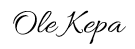
\includegraphics{"./signatures/OleKepa.png"}
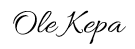
\includegraphics{"./signatures/OleKepa.png"}
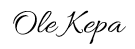
\includegraphics{"./signatures/OleKepa.png"}



\end{document}
